%----------------------------------------------------------------------
% Benchmark of the three HODLR providers available through OpenTURNS
%----------------------------------------------------------------------
\documentclass[11pt]{article}

\usepackage[margin=2.4cm]{geometry}
\usepackage{booktabs}
\usepackage{multirow}
\usepackage{graphicx}
\usepackage{caption}
\usepackage{siunitx}
\usepackage{amsmath}
\usepackage{xcolor}
\usepackage{hyperref}
\usepackage{microtype}
\hypersetup{colorlinks=true, linkcolor=blue!60!black, urlcolor=blue!60!black}

\sisetup{round-mode=places}
\graphicspath{{figures/}}
%% GENERATED by make_report.py -- do not edit by hand.

\newcommand{\tabacc}{
\begin{tabular}{l l c c c c c}
\toprule
\multicolumn{2}{c}{} & \multicolumn{4}{c}{relative error vs. dense} & \\
\cmidrule(lr){3-6}
$n$ / dim & provider & gemv & solve & logdet & KL $\lambda_1$ & $c_r$ \\
\midrule
        2000 / 1D & OpenTURNS HODLR & 5.7e-16 & 9.8e-10 & 6.2e-08 & 1.4e-14 & 0.130 \\
         & OpenTURNS HMat & 4.7e-16 & 1.0e+00 & 1.3e+04 & 7.1e-15 & 0.423 \\
         & hmat-oss direct & 2.4e-14 & 2.0e-06 & -- & 9.8e-13 & 0.230 \\
        \addlinespace
        2000 / 2D & OpenTURNS HODLR & 5.9e-07 & 5.4e-07 & 1.0e-08 & 7.5e-08 & 0.213 \\
         & OpenTURNS HMat & 3.3e-07 & 2.6e-04 & 6.0e-01 & 1.9e-08 & 0.511 \\
         & hmat-oss direct & 2.9e-07 & 6.4e-07 & 3.7e-08 & 1.1e-10 & 0.380 \\
        \addlinespace
        2000 / 3D & OpenTURNS HODLR & 4.3e-07 & 5.2e-07 & 1.8e-10 & 1.0e-07 & 0.224 \\
         & OpenTURNS HMat & 1.2e-07 & 2.0e-04 & 4.0e-01 & 2.1e-08 & 0.687 \\
         & hmat-oss direct & 2.4e-07 & 2.9e-07 & 1.9e-09 & 4.9e-08 & 0.437 \\
        \addlinespace
        5000 / 1D & OpenTURNS HODLR & 7.7e-16 & 3.5e-08 & 5.0e-07 & 2.8e-14 & 0.065 \\
         & OpenTURNS HMat & 5.0e-08 & 1.0e+00 & 5.4e+04 & 3.0e-06 & 0.126 \\
         & hmat-oss direct & 9.5e-15 & 3.7e-05 & -- & 1.0e-12 & 0.066 \\
        \addlinespace
        5000 / 2D & OpenTURNS HODLR & 3.8e-05 & 1.3e-04 & 1.6e-04 & 2.1e-05 & 0.123 \\
         & OpenTURNS HMat & 9.2e-07 & 3.2e-04 & 4.5e+00 & 8.1e-07 & 0.187 \\
         & hmat-oss direct & 7.4e-06 & 3.3e-05 & 7.9e-05 & 1.3e-05 & 0.200 \\
        \addlinespace
        5000 / 3D & OpenTURNS HODLR & 3.2e-05 & 4.0e-05 & 2.4e-06 & 4.6e-06 & 0.174 \\
         & OpenTURNS HMat & 1.2e-05 & 2.0e-04 & 1.0e+00 & 2.4e-06 & 0.289 \\
         & hmat-oss direct & 3.8e-05 & 4.3e-05 & 4.3e-06 & 1.1e-05 & 0.249 \\
\bottomrule
\end{tabular}}

\newcommand{\tabtime}{
\begin{tabular}{l l c c c c c c c}
\toprule
\multicolumn{2}{c}{} & \multicolumn{7}{c}{wall-clock time [ms]} \\
\cmidrule(lr){3-9}
$n$ / dim & provider & assemble & Chol. & LU & gemv & solve & solveLower & logdet \\
\midrule
        2000 / 1D & OpenTURNS HODLR & 25.0 & 5.1 & 31.5 & 0.11 & 0.21 & 0.09 & 0.00 \\
         & OpenTURNS HMat & 12.3 & 10.1 & 18.9 & 0.18 & 0.26 & 0.12 & 0.00 \\
         & hmat-oss direct & 4.7 & 1.8 & 2.2 & 0.13 & 0.17 & 0.08 & 0.01 \\
        \addlinespace
        2000 / 2D & OpenTURNS HODLR & 8.6 & 18.1 & 34.6 & 0.38 & 0.38 & 0.18 & 0.00 \\
         & OpenTURNS HMat & 17.5 & 20.8 & 25.5 & 0.22 & 0.31 & 0.15 & 0.00 \\
         & hmat-oss direct & 18.9 & 7.8 & 9.9 & 0.26 & 0.31 & 0.15 & 0.01 \\
        \addlinespace
        2000 / 3D & OpenTURNS HODLR & 11.9 & 23.7 & 42.2 & 0.42 & 0.42 & 0.19 & 0.00 \\
         & OpenTURNS HMat & 21.0 & 31.3 & 31.4 & 0.34 & 0.43 & 0.21 & 0.00 \\
         & hmat-oss direct & 32.1 & 11.4 & 16.4 & 0.27 & 0.40 & 0.18 & 0.01 \\
        \addlinespace
        5000 / 1D & OpenTURNS HODLR & 196 & 17.8 & 223 & 0.37 & 0.72 & 0.33 & 0.00 \\
         & OpenTURNS HMat & 26.7 & 19.3 & 36.4 & 0.33 & 0.50 & 0.24 & 0.01 \\
         & hmat-oss direct & 9.8 & 3.3 & 4.4 & 0.25 & 0.44 & 0.16 & 0.01 \\
        \addlinespace
        5000 / 2D & OpenTURNS HODLR & 73.6 & 116 & 247 & 1.8 & 1.5 & 0.73 & 0.00 \\
         & OpenTURNS HMat & 65.4 & 94.2 & 78.3 & 0.83 & 0.83 & 0.41 & 0.01 \\
         & hmat-oss direct & 97.1 & 45.4 & 52.2 & 0.97 & 1.6 & 0.67 & 0.02 \\
        \addlinespace
        5000 / 3D & OpenTURNS HODLR & 199 & 274 & 705 & 4.4 & 3.0 & 1.5 & 0.00 \\
         & OpenTURNS HMat & 81.1 & 170 & 103 & 1.5 & 2.0 & 0.81 & 0.01 \\
         & hmat-oss direct & 181 & 75.3 & 95.2 & 1.3 & 2.3 & 1.1 & 0.02 \\
\bottomrule
\end{tabular}}

\newcommand{\tabapp}{
\begin{tabular}{l l c c c c}
\toprule
\multicolumn{2}{c}{} & \multicolumn{4}{c}{end-to-end time [ms]} \\
\cmidrule(lr){3-6}
$n$ / dim & provider & sampling & KL & log-lik. & regression \\
\midrule
        2000 / 1D & dense & -- & 319 & -- & -- \\
        2000 / 1D & OpenTURNS HODLR & 30 & 109 & 30 & 30 \\
         & OpenTURNS HMat & 23 & 91 & 22 & 23 \\
         & hmat-oss direct & 7 & 63 & 7 & 7 \\
        \addlinespace
        2000 / 2D & dense & -- & 319 & -- & -- \\
        2000 / 2D & OpenTURNS HODLR & 27 & 185 & 27 & 27 \\
         & OpenTURNS HMat & 39 & 111 & 38 & 39 \\
         & hmat-oss direct & 27 & 88 & 27 & 27 \\
        \addlinespace
        2000 / 3D & dense & -- & 320 & -- & -- \\
        2000 / 3D & OpenTURNS HODLR & 36 & 202 & 36 & 36 \\
         & OpenTURNS HMat & 53 & 147 & 53 & 53 \\
         & hmat-oss direct & 44 & 97 & 44 & 44 \\
        \addlinespace
        5000 / 1D & dense & -- & 2031 & -- & -- \\
        5000 / 1D & OpenTURNS HODLR & 214 & 511 & 214 & 214 \\
         & OpenTURNS HMat & 46 & 259 & 46 & 47 \\
         & hmat-oss direct & 13 & 175 & 13 & 14 \\
        \addlinespace
        5000 / 2D & dense & -- & 2002 & -- & -- \\
        5000 / 2D & OpenTURNS HODLR & 191 & 1071 & 190 & 191 \\
         & OpenTURNS HMat & 160 & 375 & 160 & 160 \\
         & hmat-oss direct & 144 & 393 & 143 & 144 \\
        \addlinespace
        5000 / 3D & dense & -- & 2055 & -- & -- \\
        5000 / 3D & OpenTURNS HODLR & 475 & 1592 & 474 & 476 \\
         & OpenTURNS HMat & 253 & 595 & 252 & 253 \\
         & hmat-oss direct & 258 & 506 & 257 & 259 \\
\bottomrule
\end{tabular}}

\newcommand{\tabdense}{
\begin{tabular}{l c c c c}
\toprule
config & $n_{\mathrm{grid}}$ & $\log\det A$ & $\lambda_1$ & dense KL [ms] \\
\midrule
        2000 / 1D & 2000 & -20782.8 & 47.6515 & 319 \\
        2000 / 2D & 2000 & -32.6 & 1.4528 & 319 \\
        2000 / 3D & 2000 & 0.0 & 1.0000 & 320 \\
        5000 / 1D & 5000 & -71400.8 & 119.1645 & 2031 \\
        5000 / 2D & 5000 & -988.5 & 3.1309 & 2002 \\
        5000 / 3D & 5000 & -0.0 & 1.0008 & 2055 \\
\bottomrule
\end{tabular}}


\newcommand{\ot}{OpenTURNS}

\title{Benchmark of the HODLR providers available through \ot{}\\[2mm]
\large assembly, factorization, solve, sampling and log-determinant for a Matern~5/2 covariance}
\author{}
\date{\today}
\begin{document}
\sloppy

\maketitle

\begin{abstract}
We benchmark the three providers of hierarchical (\textsc{hodlr}) linear algebra
available from the \ot{} code base for the covariance matrix of a Matern~5/2
process: the \emph{native} \ot{} \textsc{hodlr} implementation
(\texttt{HODLRMatrix}), the \ot{} \textsc{hmat} wrapper around the external
\emph{hmat-oss} library (\texttt{HMatrix}), and \emph{hmat-oss} driven directly
through its C API.  For grids of $n \in \{2000, 5000\}$ points in 1D, 2D and 3D,
target precision $\varepsilon = 10^{-6}$ and length scale $\ell = 0.01$, we
measure the wall-clock time and the numerical accuracy (with respect to a dense
reference) of the routines used by \texttt{GaussianProcess} (sampling),
\texttt{KarhunenLoeveP1Algorithm} (eigenvalues via Lanczos),
\texttt{GaussianProcessFitter} (log-likelihood) and
\texttt{GaussianProcessRegression} (solve).  The direct \emph{hmat-oss} path is
the fastest for factorization and solves; the native \ot{}
\textsc{hodlr} is the most robust numerically, in particular for the
log-determinant and for the severely ill-conditioned 1D configurations.  The
\ot{} \textsc{hmat} path implicitly regularizes the matrix before
factorization, which makes its post-factorization solve and log-determinant
deviate from the exact values on ill-conditioned matrices.
\end{abstract}

\section{Objective}\label{sec:objective}

OpenTURNS 0.29 exposes two hierarchical matrix backends for its Gaussian-process
machinery, plus the option to use the \texttt{hmat-oss} library directly:

\begin{enumerate}
  \item \texttt{HODLRMatrix} (native, this \texttt{hodlr} branch), assembled by
        \texttt{discretizeHODLRMatrix}, used by \texttt{GaussianProcess},
        \texttt{GaussianProcessFitter}, \texttt{GaussianProcessRegression} and
        \texttt{KarhunenLoeveP1Algorithm};
  \item \texttt{HMatrix} (wrapper over \texttt{hmat-oss} v1.11.1, built with
        \texttt{OPENTURNS\_HAVE\_HMAT}), used by the same modules through
        \texttt{HMatrixFactory};
  \item \texttt{hmat-oss} v1.11.1 driven directly through its C API (the
        ``provider ceiling'' of the wrapper).
\end{enumerate}

This report compares the three providers on the covariance matrix of a Matern~5/2
process with amplitude~1, length scale $\ell = 0.01$ and nugget $10^{-8}$, on
structured grids of $n$ points in $[0,1]^d$ with $d \in \{1,2,3\}$, target
assembly/recompression precision $\varepsilon = 10^{-6}$ and (minimum) leaf size
250.  All runs are single threaded
($\texttt{OPENBLAS\_NUM\_THREADS}=\texttt{OMP\_NUM\_THREADS}=1$) on the \ot{}
\emph{build-perf} tree (\texttt{-O3}).  The accuracy is measured against a dense
reference assembled entry-by-entry and factorized with LAPACK
\texttt{dpotrf}.  Each timing is the best of three repetitions.

\section{Configuration}\label{sec:config}

The point sets are regular grids: $n$ uniformly spaced points in 1D, $k^2$ points
with $k=\lceil\sqrt n\rceil$ in 2D and $k^3$ points with $k=\lceil\sqrt[3]{n}\rceil$
in 3D (Table~\ref{tab:dense}).  The 1D covariance is extremely ill-conditioned
(the length scale $\ell=0.01$ is much larger than the spacing $\approx 2\cdot
10^{-4}$), the 2D one moderately so, while the 3D covariance is close to the
identity (Table~\ref{tab:dense}).

\begin{table}[h]
  \centering
  \caption{Grids and dense reference values (Matern~5/2, $\ell=0.01$, variance~1,
           nugget $10^{-8}$).  $\log\det A$ and $\lambda_1$ are the dense values;
           ``dense KL'' is the wall-clock time of the Lanczos reference on the
           dense matrix.}
  \label{tab:dense}
  \tabdense
\end{table}

\section{Providers and routine mapping}\label{sec:providers}

Each provider assembles the same symmetric matrix and performs the same
operations, but with different entry points:

\begin{itemize}
  \item \textbf{native \ot{} \textsc{hodlr}}: assembly through
        \texttt{discretizeHODLRMatrix} with \texttt{HODLRMatrixParameters}
        (\texttt{AssemblyEpsilon}=\texttt{RecompressionEpsilon}=$10^{-6}$,
        \texttt{MinLeafSize}=250), factorization \texttt{factorize("LLT")} or
        \texttt{factorize("LU")}, then \texttt{gemv}/\texttt{applyFactor}/
        \texttt{solve}/\texttt{solveLower}/\texttt{logDeterminant}.
  \item \textbf{\ot{} \textsc{hmat} wrapper}: \texttt{HMatrixFactory::build},
        \texttt{assemble(f, params, 'L')} with
        \texttt{CompressionMethod=AcaRandom}, \texttt{addIdentity}(nugget),
        \texttt{factorize("LLt")} or \texttt{factorize("LU")}, then
        \texttt{gemv}/\texttt{solve}/\texttt{solveLower}/\texttt{getDiagonal}.
  \item \textbf{hmat-oss direct}: same sequence through the C API
        (\texttt{libbench\_hmat2.so} shim), with median/max-dof clustering,
        \texttt{AcaRandom} compression, \texttt{hodlrsym}/\texttt{hodlr}
        factorizations.
\end{itemize}

The routines measured map to the four \ot{} modules as follows
(see \texttt{lib/src/Base/Stat/HMatrixImplementation.cxx},
\texttt{HODLRMatrixImplementation.cxx} and
\texttt{lib/src/Base/Algo/KarhunenLoeveP1Algorithm.cxx}):

\begin{itemize}
  \item \textbf{\texttt{GaussianProcess} sampling}: assemble, factorize, then
        $L z$ (\texttt{applyFactor} for \textsc{hodlr}, \texttt{gemv} for
        \textsc{hmat}).
  \item \textbf{\texttt{KarhunenLoeveP1Algorithm}}: assemble; for
        \textsc{hodlr} the matrix is \textsc{lu}-factorized and the Lanczos
        iterations use the factorized \texttt{gemv}; for \textsc{hmat} and for
        \texttt{hmat-oss} the Lanczos iterations use the assembled matrix.
        The reported ``KL time'' is the full Lanczos run (300 iterations,
        full re-orthogonalization, 10 eigenvalues).
  \item \textbf{\texttt{GaussianProcessFitter}} (log-likelihood): assemble,
        factorize, \texttt{solveLower}(data), \texttt{solveLower}(design) and
        the log-determinant (native \textsc{hodlr}: \texttt{logDeterminant};
        \textsc{hmat}: \texttt{getDiagonal} + $\sum\log d_{ii}$;
        \texttt{hmat-oss}: \texttt{logdet}).
  \item \textbf{\texttt{GaussianProcessRegression}}: assemble, factorize,
        \texttt{solve}.
\end{itemize}

\section{Results}\label{sec:results}

\subsection{Timings}\label{sec:timings}

Table~\ref{tab:time} reports the per-routine wall-clock times; Figures
\ref{fig:assemble}--\ref{fig:kl} show the assembly, Cholesky, LU and solve times
and the end-to-end KL run.

\begin{table}[h]
  \centering
  \caption{Wall-clock times (best of 3, single thread).  ``gemv'' is the
           matrix--vector product $A v$ on the (re)assembled matrix, ``Chol.''
           the LLT/LLt factorization, ``logdet'' the log-determinant extraction
           (native \textsc{hodlr}: stored value; \textsc{hmat}:
           \texttt{getDiagonal}; \texttt{hmat-oss}: \texttt{logdet}).  ``--''
           means the operation is not available or the number is not finite.}
  \label{tab:time}
  \tabtime
\end{table}

\begin{table}[h]
  \centering
  \caption{End-to-end timings of the four application-level workflows (sum of
           the involved routines; sampling = assemble + factorize +
           $L z$).  The ``dense'' row is the Lanczos reference on the dense
           matrix.}
  \label{tab:app}
  \tabapp
\end{table}

\begin{figure}[h]
  \centering
  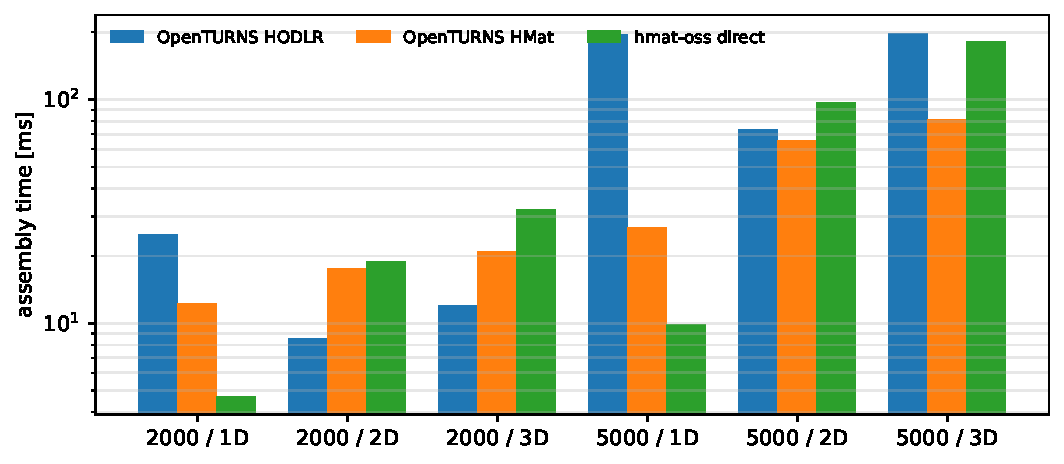
\includegraphics[width=0.95\linewidth]{assemble}
  \caption{Assembly time (log scale).}
  \label{fig:assemble}
\end{figure}

\begin{figure}[h]
  \centering
  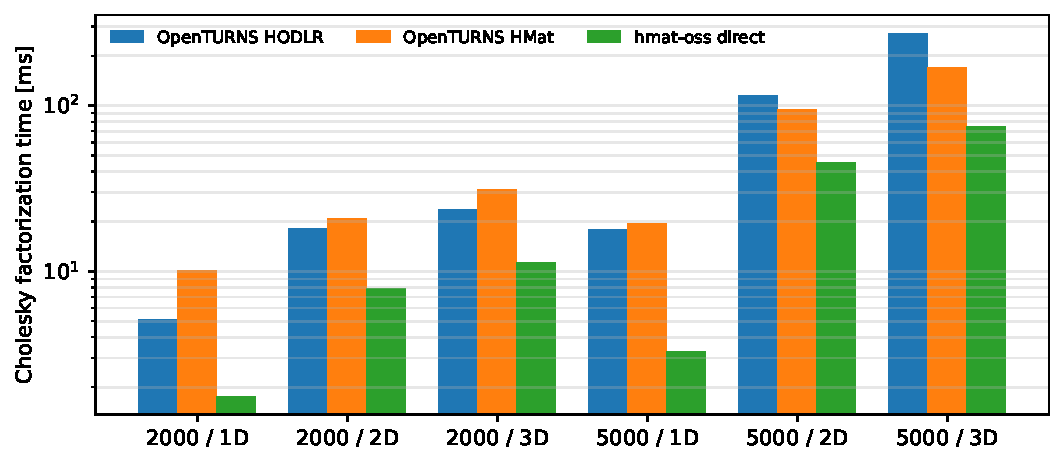
\includegraphics[width=0.95\linewidth]{factorize_llt}
  \caption{Cholesky (LLT/LLt) factorization time (log scale).}
  \label{fig:llt}
\end{figure}

\begin{figure}[h]
  \centering
  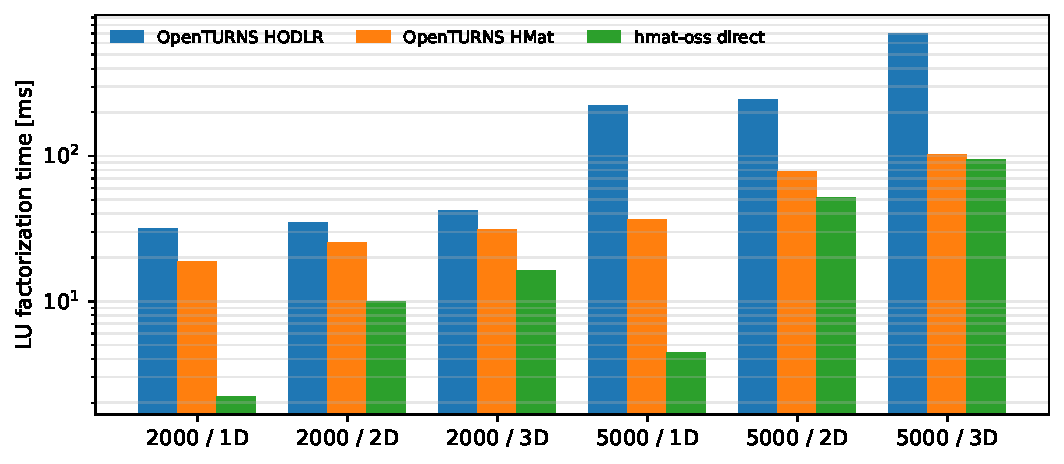
\includegraphics[width=0.95\linewidth]{factorize_lu}
  \caption{LU factorization time (log scale).}
  \label{fig:lu}
\end{figure}

\begin{figure}[h]
  \centering
  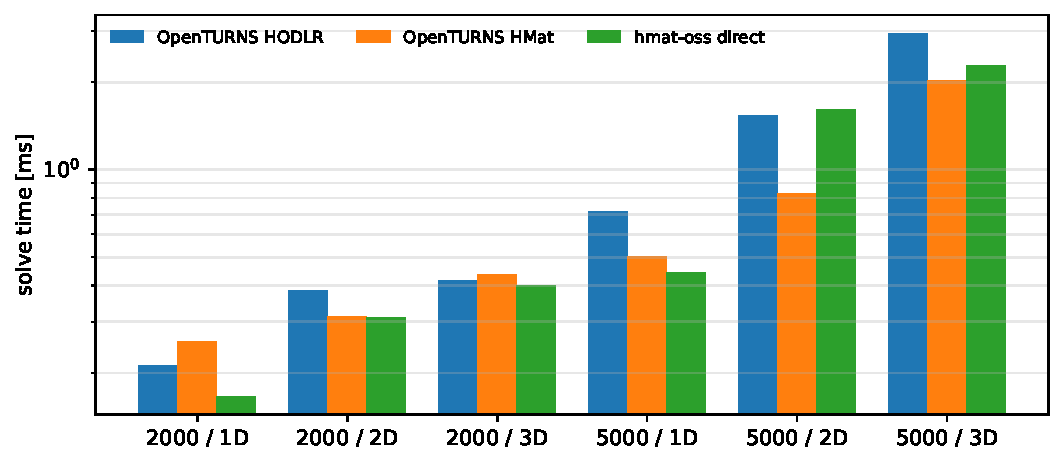
\includegraphics[width=0.95\linewidth]{solve}
  \caption{Single right-hand-side solve time (log scale).}
  \label{fig:solve}
\end{figure}

\begin{figure}[h]
  \centering
  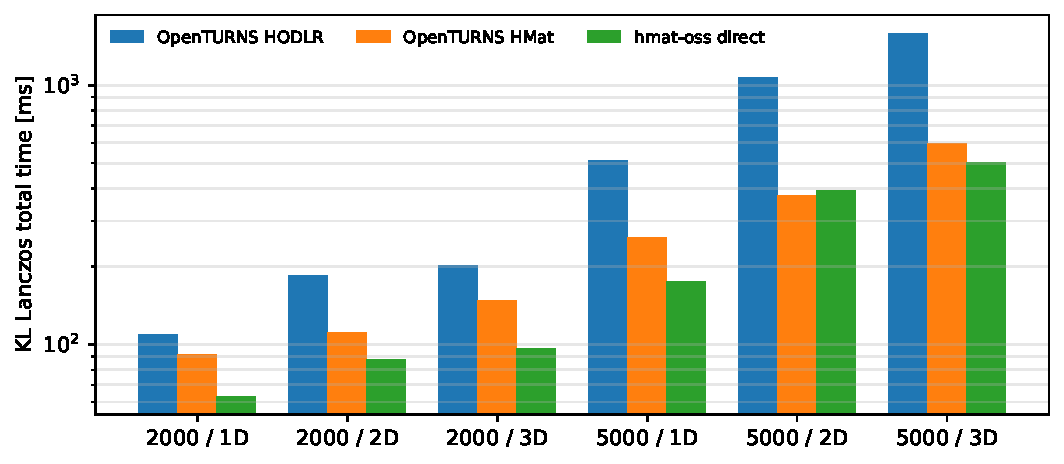
\includegraphics[width=0.95\linewidth]{kl}
  \caption{End-to-end KL Lanczos run (300 matrix--vector products; log scale).}
  \label{fig:kl}
\end{figure}

\subsection{Accuracy}\label{sec:accuracy}

Table~\ref{tab:acc} reports the relative errors with respect to the dense
reference: the matvec $A v$ (``gemv''), the solve (``solve''), the
log-determinant (``logdet'') and the largest eigenvalue returned by the KL
Lanczos (``KL $\lambda_1$''), together with the compression ratio
$c_r = $ stored coefficients $/\, n^2$.

\begin{table}[h]
  \centering
  \caption{Relative errors vs.\ the dense reference.  The ``gemv'' column is the
           matvec accuracy of the assembled matrix, which is the meaningful
           comparison for all providers.  ``--'' means not finite.}
  \label{tab:acc}
  \tabacc
\end{table}

\section{Findings}\label{sec:findings}

\paragraph{Assembly.}
The native \ot{} \textsc{hodlr} assembly is fastest in 2D/3D at $n=2000$
($8$--$12$\,ms) but the slowest in 1D at $n=5000$ ($196$\,ms), while
\texttt{hmat-oss} shows the opposite trend ($4.7$\,ms in 1D/$n=2000$,
$181$\,ms in 3D/$n=5000$).  The \ot{} \textsc{hmat} assembly is the middle
option everywhere.  The native \ot{} \textsc{hodlr} reaches the smallest
compression ratios (up to $0.065$ vs.\ $0.066$--$0.437$), i.e.\ it is the most
storage-efficient.

\paragraph{Cholesky factorization.}
\texttt{hmat-oss} is consistently the fastest ($1.8$--$75$\,ms), followed by the
native \ot{} \textsc{hodlr} in 1D ($5.1$ and $17.8$\,ms) and by the \ot{}
\textsc{hmat} wrapper in 2D/3D.  The two \ot{} entry points are within
$\approx 1.6\times$ of each other everywhere except the 1D case where the
native \textsc{hodlr} is $\approx 2\times$ faster than the wrapper.

\paragraph{LU factorization.}
The native \ot{} \textsc{hodlr} \textsc{lu} path is by far the slowest
operation of the whole benchmark: $6\times$--$12\times$ slower than its own
Cholesky ($223$\,ms at $n=5000$ in 1D, $704$\,ms in 3D).  \texttt{hmat-oss}
\textsc{hodlr} (LU) and the \ot{} \textsc{hmat} \textsc{lu} stay close to their
symmetric factorization cost.  Since \texttt{KarhunenLoeveP1Algorithm} uses the
\textsc{lu} factorization on the \textsc{hodlr} path, this is where the native
backend is penalized; nevertheless its end-to-end KL time remains $4\times$
faster than the dense Lanczos at $n=5000$ in 1D.

\paragraph{Solves.}
All three providers solve in well under $3$\,ms at $n=5000$; the 
\texttt{hmat-oss} direct path is the fastest.  The accuracy of the solve is
limited by the conditioning: for the ill-conditioned 1D matrices the native
\textsc{hodlr} and \texttt{hmat-oss} reach $3.5\times10^{-8}$ and
$3.7\times10^{-5}$, respectively, at $n=5000$.

\paragraph{Log-determinant.}
The native \ot{} \textsc{hodlr} \texttt{logDeterminant} is both the cheapest
(stored at factorization) and the most accurate ($10^{-10}$--$2.4\times10^{-6}$).
The \texttt{hmat-oss} \texttt{logdet} follows the documented convention of
returning $\log|\det L|=\frac12\log\det A$ for the symmetric (HODLRSYM)
factorization and must be doubled by the caller; once doubled it is accurate to
$10^{-9}$--$8\times10^{-5}$ in 2D/3D but returns $-\infty$ on the 1D
configurations, where the leaf LLT produces a non-positive diagonal.  The \ot{}
\textsc{hmat} wrapper extracts the log-determinant from
\texttt{getDiagonal}, but on the \emph{regularized} factor (see below).

\paragraph{Implicit regularization of the \ot{} \textsc{hmat} path.}
\texttt{HMatrixImplementation::factorize} computes $\lambda_{\max}$ by power
iteration and calls \texttt{addIdentity($\lambda$)} with
$\lambda = 2\,\lambda_{\max}\,\cdot$\texttt{HMatrix-RegularizationEpsilon}
(default $10^{-4}$), doubling $\lambda$ and retrying while the hmat-oss
factorization fails.  The assembled matrix itself is exact ($A v$ error
$\le 5\times10^{-8}$), but all post-factorization operations solve or
factorize $A+\lambda I$ rather than $A$.  For the 1D matrices ($\lambda \approx
9.5\times10^{-3}$ at $n=2000$) this shifts the solve relative error to
$\approx 1$ and the log-determinant by up to $5.4\times10^{4}$; for the
well-conditioned 2D/3D cases the deviation drops to $10^{-4}$--$1$.  The native
\ot{} \textsc{hodlr} has the same mechanism
(\texttt{HODLRMatrix-RegularizationEpsilon}) but only applies the shift if the
unshifted factorization fails, which never happened here.

\paragraph{Compression method.}
\texttt{hmat-oss} compression with \texttt{AcaPlus} at $\varepsilon=10^{-6}$ is
surprisingly inaccurate on 2D kernels (matvec error $\approx 2\times10^{-2}$ at
$n=2000$, whereas SVD/AcaFull/AcaPartial/AcaRandom all give $\approx
10^{-10}$).  All runs of this report therefore use \texttt{AcaRandom}, which is
also the default \texttt{HMatrix-CompressionMethod} of \ot{}.

\paragraph{Post-factorization gemv semantics.}
After a Cholesky factorization the \texttt{gemv} of the native \ot{}
\textsc{hodlr} returns $A v$ (it uses the factorized blocks to reconstruct the
matvec), whereas \texttt{hmat-oss} returns $L v$.  Both are correct uses for
their respective callers: \texttt{GaussianProcess} sampling relies on
$L z$ (\texttt{applyFactor} for \textsc{hodlr}, \texttt{gemv} for
\textsc{hmat}).

\paragraph{Accuracy at the requested precision.}
At $\varepsilon=10^{-6}$ the three providers meet the target on the matvec and
on the KL eigenvalues for all configurations ($10^{-16}$--$4\times10^{-5}$).
The solve and log-determinant accuracies are bounded by $\kappa\,\varepsilon$
for the native and \texttt{hmat-oss} paths, which explains the larger errors on
the 1D (near-singular) matrices; the \ot{} \textsc{hmat} solve/log-determinant
are additionally shifted by the regularization described above.

\section{Conclusion}\label{sec:conclusion}

The \texttt{hmat-oss} direct path is the fastest provider for factorization and
linear algebra, at the price of two documented caveats (halved HODLRSYM
log-determinant and its failure on severely ill-conditioned matrices, and the
unreliable \texttt{AcaPlus} compression in 2D).  The native \ot{}
\textsc{hodlr} is the most robust numerically -- the only provider that keeps
the log-determinant accurate on the 1D matrices -- and the most
storage-efficient, but its \textsc{lu} factorization is an order of magnitude
slower than its Cholesky, which penalizes the \texttt{KarhunenLoeveP1Algorithm}
workflow.  The \ot{} \textsc{hmat} wrapper is a convenient middle ground whose
main caveat is the implicit regularization shift applied before factorization.

\appendix
\section*{Reproduction}\label{sec:repro}

\begin{itemize}
  \item Harness: \texttt{/tmp/opencode/hodlrbench/hodlr\_compare.cxx}
        (OpenTURNS side) and \texttt{bench\_hmat2.c} (hmat-oss C shim);
        raw results in \texttt{/tmp/opencode/hodlrbench/results/run\_*.json}.
  \item Report data/figures: \texttt{make\_report.py} (this directory).
  \item Build: \texttt{cmake --preset=linux-debug} then
        \texttt{cmake --build build-perf --target install} (the \texttt{-O3}
        build used for benchmarking).
\end{itemize}

\end{document}
